\chapter{Potentiels thermodynamiques}\label{ch:b2:thermodynamic-potentials}

Étirez vivement un élastique et portez-le à vos lèvres~: il est chaud~;
laissez-le se contracter et il est froid. Suspendez-lui un poids et chauffez-le au
sèche-cheveux~: il \emph{raccourcit}. Aucun ressort d'acier ne se comporte ainsi, et la
raison est que la tension d'un élastique n'est pas affaire d'énergie mais
d'entropie --- les chaînes étirées ont moins de façons de se ranger.
Pour raisonner sur de telles choses il faut savoir ce que fait un système à
température fixée, ou à température et pression fixées, et
quel travail on peut en tirer~: questions auxquelles l'énergie interne et
l'entropie ne répondent que gauchement, parce qu'elles parlent la langue d'un
système isolé. Ce chapitre introduit les deux fonctions bâties pour les
conditions du laboratoire, l'\emph{\omterm{def:b2:thermodynamic-potentials:FG}{énergie libre} de Helmholtz} $F = U -
TS$ et l'\emph{\omterm{def:b2:thermodynamic-potentials:FG}{enthalpie libre} de Gibbs} $G = H - TS$, montre qu'elles
mesurent le travail récupérable et décroissent vers l'équilibre, extrait
de leurs différentielles les relations de Maxwell qui lient des grandeurs
qu'on n'aurait pas crues liées, et applique le tout à
l'équilibre de deux phases, où $G$ décide quelle phase l'emporte et
redonne la formule de Clapeyron.

\begin{omfigure}
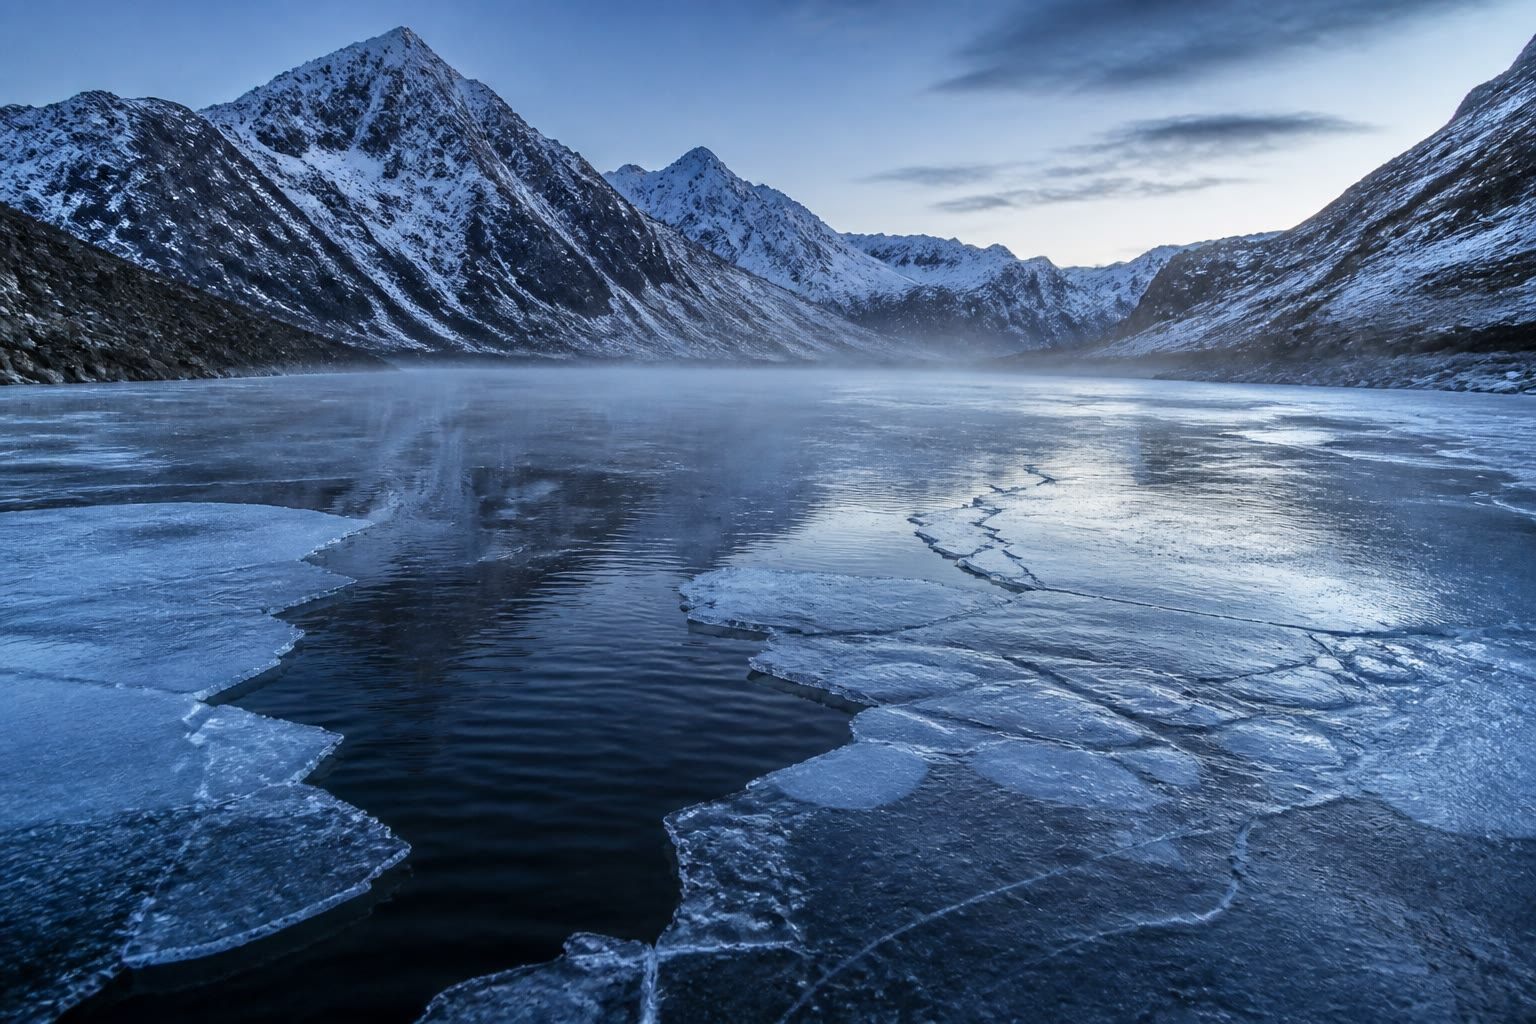
\includegraphics[width=0.58\linewidth]{images/book4/ai/b4-28-ice-lake-dawn.jpg}

{\small Glace et eau coexistant sur un lac à l'aube~: au point de
fusion les deux phases ont la même \omterm{def:b2:thermodynamic-potentials:FG}{enthalpie libre} par kilogramme, et un
petit changement de pression ou de température fait pencher la balance --- la
pente de Clapeyron dit de combien.}
\end{omfigure}

\section{L'identité fondamentale et ses variables}

\begin{proposition}[Identité fondamentale]\label{prop:b2:thermodynamic-potentials:identity}
Pour un système fermé de composition fixée, l'énergie interne,
vue comme fonction de l'entropie et du volume, vérifie
\[
\dd U = T\,\dd S - P\,\dd V, \qquad
T = \Big(\frac{\partial U}{\partial S}\Big)_V, \quad
P = -\Big(\frac{\partial U}{\partial V}\Big)_S ,
\]
et l'\omterm{thm:b2:open-systems:firstlaw}{enthalpie} $H = U + PV$ vérifie $\dd H = T\,\dd S + V\,\dd P$.
Chaque fonction, dans ses \emph{variables naturelles}\index{variables naturelles} --- $(S,V)$ pour $U$, $(S,P)$ pour $H$ --- contient toute la
thermodynamique du système~: ses dérivées partielles donnent les autres
variables d'état. Le second principe désigne l'équilibre d'un système
isolé ($U$, $V$ fixés) comme l'état de $S$ maximale.
\end{proposition}

\begin{proof}
Le premier principe pour une transformation réversible, $\dd U = \delta Q_{\text{rev}}
+ \delta W_{\text{rev}} = T\,\dd S - P\,\dd V$, ne fait intervenir que des fonctions
d'état et vaut donc pour toute variation infinitésimale entre
états d'équilibre. Ajouter $\dd(PV)$ pour $H$.
\end{proof}

\begin{remark}[Pourquoi de nouvelles fonctions]\label{rem:b2:thermodynamic-potentials:why}
Les expériences ne se font pas à entropie fixée. Le ballon d'un chimiste est à
la température de la pièce et à la pression de l'atmosphère~; un
piston dans un thermostat travaille à $T$ fixée. On veut des fonctions dont les
\omterm{prop:b2:thermodynamic-potentials:identity}{variables naturelles} sont $(T,V)$ et $(T,P)$, et qui jouent, dans ces
conditions, le rôle que $S$ joue pour un système isolé~: dire
dans quel sens le système évolue et quel travail il peut donner. Une
\emph{transformée de Legendre} --- retrancher $TS$ pour échanger $S$ contre $T$ comme
variable indépendante --- les construit.
\end{remark}

\section{Énergie libre et enthalpie libre}

\begin{definition}[Énergie libre de Helmholtz, enthalpie libre de Gibbs]\label{def:b2:thermodynamic-potentials:FG}
\[
F = U - TS \quad\text{(\emph{énergie libre}\index{énergie libre})}, \qquad
G = H - TS = U + PV - TS \quad\text{(\emph{enthalpie libre}\index{enthalpie libre})}.
\]
Toutes deux sont des fonctions d'état extensives, mesurées en joules.
\end{definition}

\begin{theorem}[Différentielles et grandeurs dérivées]\label{thm:b2:thermodynamic-potentials:dFdG}
\[
\dd F = -S\,\dd T - P\,\dd V, \qquad
\dd G = -S\,\dd T + V\,\dd P ;
\]
d'où, dans les \omterm{prop:b2:thermodynamic-potentials:identity}{variables naturelles} $(T,V)$ de $F$ et $(T,P)$ de $G$,
\[
S = -\Big(\frac{\partial F}{\partial T}\Big)_V, \quad
P = -\Big(\frac{\partial F}{\partial V}\Big)_T, \qquad
S = -\Big(\frac{\partial G}{\partial T}\Big)_P, \quad
V = \Big(\frac{\partial G}{\partial P}\Big)_T ,
\]
et (Gibbs--Helmholtz) $U = F - T(\partial F/\partial T)_V =
-T^2\,\partial(F/T)/\partial T$, $H = -T^2\,\partial(G/T)/\partial T$.
Connaître $F(T,V)$ ou $G(T,P)$, c'est tout connaître~: l'équation
d'état, l'entropie, l'énergie, les capacités thermiques.
\end{theorem}

\begin{proof}
$\dd F = \dd U - T\dd S - S\dd T = -S\dd T - P\dd V$~; de même pour $G$
à partir de $\dd H$. On lit les dérivées partielles~; pour Gibbs--Helmholtz,
$F - T\,\partial_TF = F + TS = U$ et $\partial_T(F/T) = (T\partial_TF -
F)/T^2 = -U/T^2$.
\end{proof}

\begin{example}[Le gaz parfait]\label{ex:b2:thermodynamic-potentials:perfect}
Pour $n$ moles, $U = nc_{V}T + U_0$ et $S = nc_V\ln T + nR\ln V + S_0$
donnent $F(T,V) = -nRT\ln V + f(T)$~: alors $P = -\partial_VF = nRT/V$
--- l'équation d'état sort de $F$ --- et $S = -\partial_TF$
redonne l'entropie. Dans les variables $(T,P)$, $G(T,P) = nRT\ln P +
g(T)$, donc $V = \partial_PG = nRT/P$, et l'\omterm{def:b2:thermodynamic-potentials:FG}{enthalpie libre} \emph{molaire}
$\mu(T,P) = \mu^\circ(T) + RT\ln(P/P^\circ)$ --- le \emph{potentiel
chimique}\index{potentiel chimique} du gaz, qui croît avec sa
pression~: le gaz s'écoule des $\mu$ élevés vers les bas, ici des hautes vers les basses
pressions.
\end{example}

\section{Travail maximal et sens de l'évolution}

\begin{theorem}[Transformations monothermes]\label{thm:b2:thermodynamic-potentials:monothermal}
Un système échangeant de la chaleur avec un seul thermostat à $T_0$, et dont les
températures initiale et finale valent $T_0$, reçoit au cours de toute
transformation le travail
\[
W \ge \Delta F , \qquad\text{c'est-à-dire}\qquad W_{\text{récupéré}} = -W \le -\Delta F :
\]
la diminution de $F$ est le \emph{travail maximal récupérable} du
système à température fixée (atteint pour une transformation réversible) ---
d'où l'énergie «~libre~»~: la part de $U$ convertible en travail, le
reste, $TS$, étant lié. Si de plus la transformation est monobare
(pression $P_0$ à l'extérieur, pressions initiale et finale $P_0$), le travail
\emph{autre que celui de l'atmosphère} (\omterm{def:b2:open-systems:cv}{travail utile}, par exemple électrique)
vérifie $W_{\text{u}} \ge \Delta G$~: $-\Delta G$ est le \omterm{def:b2:open-systems:cv}{travail utile} maximal
récupérable à $T$ et $P$ fixées (le travail d'une pile à combustible, d'une
batterie).
\end{theorem}

\begin{proof}
Premier principe~: $\Delta U = W + Q$. Second principe avec un seul thermostat~: $\Delta S
= Q/T_0 + S_{\text{c}}$, $S_{\text{c}} \ge 0$, donc $Q \le T_0\Delta S$. D'où
$W = \Delta U - Q \ge \Delta U - T_0\Delta S = \Delta(U - T_0S) = \Delta F$, en utilisant
$T = T_0$ aux deux bouts. En séparant le travail de l'atmosphère $-P_0\Delta V$,
$W = W_{\text{u}} - P_0\Delta V$ et $W_{\text{u}} \ge \Delta U + P_0
\Delta V - T_0\Delta S = \Delta G$.
\end{proof}

\begin{theorem}[Critères d'évolution et d'équilibre]\label{thm:b2:thermodynamic-potentials:criteria}
Un système maintenu à $T$ et $V$ fixés et ne recevant aucun travail ne peut
évoluer qu'en faisant \emph{décroître $F$}~; son équilibre est l'état de
$F$ minimale. Un système maintenu à $T$ et $P$ fixés et ne recevant aucun \omterm{def:b2:open-systems:cv}{travail
utile} ne peut évoluer qu'en faisant \emph{décroître $G$}~; son équilibre est
l'état de $G$ minimale. (Plus généralement, pour un système en contact avec
un milieu à $T_0$, $P_0$, la quantité $U - T_0S + P_0V$ décroît.)
\end{theorem}

\begin{proof}
Prendre $W = 0$ (resp.\ $W_{\text{u}} = 0$) dans le théorème précédent~: $\Delta F
\le 0$ (resp.\ $\Delta G \le 0$), avec égalité pour une évolution réversible,
c'est-à-dire d'équilibre.
\end{proof}

\begin{example}[Détente isotherme, réelle et idéale]\label{ex:b2:thermodynamic-potentials:expansion}
Une mole de gaz à \qty{300}{K} se détend de \qty{1}{L} à \qty{10}{L} au
contact du thermostat~: $\Delta F = -RT\ln 10 = \qty{-5.7}{kJ}$. Une
détente réversible récupère \qty{5.7}{kJ}~; une détente contre
l'atmosphère à \qty{1}{bar} ne récupère que $P_0\Delta V = \qty{0.9}{kJ}$~; une
détente libre dans le vide, rien. Les \qty{5.7}{kJ} sont le maximum
que le gaz et son thermostat peuvent donner pour ce changement d'état, si
ingénieuse que soit la machine.
\end{example}

\section{Relations de Maxwell}

\begin{theorem}[Relations de Maxwell]\label{thm:b2:thermodynamic-potentials:maxwell}
Parce que $\dd F$ et $\dd G$ sont des différentielles exactes (théorème de Schwarz
sur les dérivées secondes croisées),
\[
\Big(\frac{\partial S}{\partial V}\Big)_T = \Big(\frac{\partial P}{\partial T}\Big)_V,
\qquad
\Big(\frac{\partial S}{\partial P}\Big)_T = -\Big(\frac{\partial V}{\partial T}\Big)_P .
\]
Elles expriment l'immesurable (comment l'entropie varie avec le volume ou la
pression à température fixée) au moyen de l'équation d'état. Deux
conséquences~:
\[
\Big(\frac{\partial U}{\partial V}\Big)_T = T\Big(\frac{\partial P}{\partial T}\Big)_V - P,
\qquad
C_P - C_V = T\Big(\frac{\partial P}{\partial T}\Big)_V\Big(\frac{\partial V}{\partial T}\Big)_P
= \frac{TV\alpha^2}{\kappa_T} ,
\]
avec $\alpha = V^{-1}(\partial V/\partial T)_P$ le coefficient de dilatation et
$\kappa_T = -V^{-1}(\partial V/\partial P)_T$ la compressibilité isotherme.
\end{theorem}

\begin{proof}
$\partial^2F/\partial T\partial V$ calculé dans les deux ordres~: $-\partial_VS =
-\partial_TP$. De même pour $G$. Puis $\dd U = T\dd S - P\dd V$ à $T$ fixée
donne $(\partial_VU)_T = T(\partial_VS)_T - P$~; et $C_P - C_V$ découle
de l'écriture $S(T,V(T,P))$~: $(\partial_TS)_P = (\partial_TS)_V +
(\partial_VS)_T(\partial_TV)_P$, multipliée par $T$.
\end{proof}

\begin{example}[Ce que révèlent ces relations]\label{ex:b2:thermodynamic-potentials:reveal}
Pour un gaz parfait, $T(\partial_TP)_V - P = 0$~: l'énergie ne dépend pas
du volume (loi de Joule retrouvée) et $C_P - C_V = nR$. Pour un gaz de van
der Waals, $(\partial_VU)_T = a/V_{\text{m}}^2$~: la pression interne des
attractions. Pour l'eau liquide, $(\partial_TP)_V = \alpha/\kappa_T = 2.1
\times 10^{-4}/4.6 \times 10^{-10} = \qty{4.6e5}{Pa/K}$~: chauffer d'un kelvin de l'eau dans un
récipient rigide et plein élève la pression de \qty{4.6}{bar}
(ne jamais fermer une bouteille pleine), et $(\partial_VU)_T \approx \qty{1400}{bar}$ ---
la cohésion du liquide~; pourtant $c_P - c_V = Tv\alpha^2/\kappa_T \approx
\qty{30}{J/kg/K}$, moins de $1\%$ de $c_P$~: pour la matière condensée les deux
capacités thermiques coïncident presque.
\end{example}

\begin{proposition}[Élasticité entropique du caoutchouc]\label{prop:b2:thermodynamic-potentials:rubber}
Pour un élastique de longueur $L$ sous la tension $f$, $\dd U = T\dd S + f\dd L$
et $\dd F = -S\dd T + f\dd L$, de sorte que $(\partial S/\partial L)_T =
-(\partial f/\partial T)_L$ et $(\partial U/\partial L)_T = f - T(\partial f/
\partial T)_L$. Le caoutchouc obéit, en bonne approximation, à $f = T\,\varphi(L)$
avec $\varphi > 0$ pour $L > L_0$~: alors $(\partial U/\partial L)_T = 0$ ---
l'énergie ne change pas quand on étire --- et $(\partial S/\partial L)_T =
-\varphi(L) < 0$~: la tension est \emph{entropique}, $f = -T(\partial S/\partial
L)_T$, l'élastique tire en arrière parce que ses chaînes étirées ont moins de
configurations. Conséquences~: étiré isothermiquement il dégage de la chaleur
($Q = T\Delta S < 0$)~; étiré adiabatiquement il s'échauffe~; chauffé sous
charge constante il se contracte ($f/T$ fixé signifie $\varphi(L)$ fixé, donc à
$f$ fixé, $\varphi$ doit baisser quand $T$ monte).
\end{proposition}

\begin{proof}
Relation de Maxwell tirée de $\dd F$~; le reste est une substitution.
L'origine microscopique est la marche au hasard du \cref{ch:b2:particle-diffusion}~:
une chaîne de $N$ maillons de longueur $a$ a sa distance bout à bout
distribuée en gaussienne de variance $Na^2$, de sorte que le nombre de
configurations à l'extension $L$ vaut $\Omega \propto \eu^{-L^2/2Na^2}$, $S = S_0 -
k_BL^2/2Na^2$ et $f = k_BTL/Na^2$~: un ressort dont la raideur est
\emph{proportionnelle à la température}.
\end{proof}

\begin{omfigure}
\begin{tikzpicture}
  \begin{axis}[omaxis, width=6.2cm, height=4.4cm, xmin=0, xmax=400, ymin=0, ymax=1.25,
    xlabel={$T$ (\unit{K})}, ylabel={$f$ (u.a.)}, xtick={100,200,300}, ytick=\empty, clip=false]
    \addplot[omDef, thick, domain=0:380] {x/300};
    \addplot[omDef, thick, domain=0:380] {0.6*x/300};
    \node[font=\scriptsize, omDef, anchor=west] at (axis cs:300,1.05) {$L - L_0$ grand};
    \node[font=\scriptsize, omDef, anchor=west] at (axis cs:300,0.5) {petit};
    \node[font=\scriptsize] at (axis cs:120,1.1) {caoutchouc~: $f \propto T$};
  \end{axis}
  \begin{axis}[omaxis, width=6.2cm, height=4.4cm, xmin=0, xmax=400, ymin=0, ymax=1.25, xshift=6.6cm,
    xlabel={$T$ (\unit{K})}, ylabel={$f$ (u.a.)}, xtick={100,200,300}, ytick=\empty, clip=false]
    \addplot[omExo, thick, domain=0:380] {1.0-0.0004*x};
    \addplot[omExo, thick, domain=0:380] {0.6-0.00024*x};
    \node[font=\scriptsize] at (axis cs:200,1.15) {acier~: $f$ presque indépendant de $T$};
  \end{axis}
\end{tikzpicture}

{\small Tension à extension fixée en fonction de la température. À gauche~: le caoutchouc,
$f \propto T$ --- la tension est entropique, $(\partial f/\partial T)_L > 0$,
donc l'étirement abaisse l'entropie et l'élastique s'échauffe. À droite~: un ressort
d'acier, dont la tension vient de l'énergie des liaisons et baisse légèrement
à mesure que le métal s'adoucit.}
\end{omfigure}

\section{Équilibre entre deux phases}

\begin{theorem}[Condition de coexistence]\label{thm:b2:thermodynamic-potentials:coexistence}
Un corps pur à $T$ et $P$ fixées, partagé entre deux phases de
masses $m_1$, $m_2$ d'\omterm{def:b2:thermodynamic-potentials:FG}{enthalpies libres} massiques $g_1(T,P)$,
$g_2(T,P)$, a $G = m_1g_1 + m_2g_2$~; à l'équilibre $G$ est minimale, donc
\begin{itemize}
\item si $g_1 < g_2$ toute la matière passe dans la phase 1 (la phase stable
      est celle de $g$ \emph{plus basse})~;
\item les deux phases ne coexistent que là où
      \[
      g_1(T,P) = g_2(T,P) ,
      \]
      relation entre $T$ et $P$~: la courbe de coexistence du diagramme
      de phases.
\end{itemize}
Le long de cette courbe (Clapeyron),
\[
\frac{\dd P}{\dd T} = \frac{s_2 - s_1}{v_2 - v_1} = \frac{L_{1\to2}}{T\,(v_2 - v_1)} .
\]
\end{theorem}

\begin{proof}
$\dd G = (g_1 - g_2)\dd m_1$ à $T$, $P$ fixées (avec $m_1 + m_2$ fixé)~:
$G$ décroît quand la masse passe dans la phase de $g$ plus basse, jusqu'à ce que cette
phase soit seule ou que $g_1 = g_2$. Différentions $g_1 = g_2$ le long de la
courbe avec $\dd g = -s\,\dd T + v\,\dd P$ pour chaque phase~: $-s_1\dd T +
v_1\dd P = -s_2\dd T + v_2\dd P$~; et $s_2 - s_1 = L/T$ puisque la transition
à $T$, $P$ fixées est réversible. Le volume de première année tirait cette formule
d'un cycle de Carnot~; ici elle tombe de $G$.
\end{proof}

\begin{omfigure}
\begin{tikzpicture}
  \begin{axis}[omaxis, width=8.6cm, height=5cm, xmin=0, xmax=10, ymin=-4.6, ymax=1.2,
    xlabel={$T$}, ylabel={$g$}, xtick=\empty, ytick=\empty, clip=false]
    \addplot[omExo, thick, domain=0:10] {0.6-0.18*x};
    \addplot[omDef, thick, domain=0:10] {1.0-0.30*x};
    \addplot[omThm, thick, domain=0:10] {3.0-0.70*x};
    \draw[dashed, gray] (axis cs:3.33,0.9) -- (axis cs:3.33,-1.0);
    \draw[dashed, gray] (axis cs:5.0,0.9) -- (axis cs:5.0,-1.2);
    \node[font=\scriptsize, below] at (axis cs:3.33,-1.0) {$T_{\text{fus}}$};
    \node[font=\scriptsize, below] at (axis cs:5.0,-1.2) {$T_{\text{vap}}$};
    \node[font=\scriptsize, omExo, anchor=west] at (axis cs:8.2,-0.6) {solide};
    \node[font=\scriptsize, omDef, anchor=west] at (axis cs:8.2,-1.6) {liquide};
    \node[font=\scriptsize, omThm, anchor=west] at (axis cs:8.2,-3.5) {gaz};
    \node[font=\scriptsize] at (axis cs:3.0,-3.9) {pente $= -s$~: la plus raide pour le gaz};
  \end{axis}
\end{tikzpicture}

{\small \omterm{def:b2:thermodynamic-potentials:FG}{Enthalpie libre} massique des trois phases à pression
fixée~: chacune baisse avec la température selon la pente $-s$, le gaz le
plus vite~; la phase stable est la ligne la plus basse, et les transitions ont lieu
là où les lignes se croisent. Les branches supérieures au-delà d'un croisement sont les
états métastables (liquide surfondu, liquide surchauffé).}
\end{omfigure}

\begin{example}[L'eau~: pentes et métastabilité]\label{ex:b2:thermodynamic-potentials:water}
Fusion~: $L = \qty{334}{kJ/kg}$, $v_{\text{liq}} - v_{\text{glace}} = -\qty{9.1e-5}{m^3/kg}$~:
$\dd P/\dd T = \qty{-1.3e7}{Pa/K}$, \emph{négative} --- la glace fond sous
pression, mais à raison de \qty{130}{bar} par kelvin~: les \qty{70}{bar} d'un patineur n'abaissent
le point de fusion que d'un demi-degré (le patinage marche par frottement et
par une couche superficielle préfondue), tandis que les \qty{270}{bar} sous trois
kilomètres de calotte en font fondre la base et la laissent glisser. Vaporisation à
\qty{100}{\celsius}~: $L = \qty{2.26}{MJ/kg}$, $\Delta v = \qty{1.67}{m^3/kg}$~:
\qty{3.6}{kPa/K} --- \qty{92}{\celsius} à \qty{0.7}{bar} en montagne,
\qty{120}{\celsius} dans une cocotte-minute à \qty{2}{bar}. Au-dessous de
\qty{0}{\celsius}, l'eau liquide a $g_{\text{liq}} - g_{\text{glace}} \approx
(L/T_{\text{fus}})(T_{\text{fus}} - T) = \qty{1.2}{kJ/kg}$ par kelvin de
surfusion~: elle est métastable, non instable, et les gouttelettes pures des
nuages restent liquides jusqu'à \qty{-40}{\celsius} faute de germe.
\end{example}

\begin{omfigure}
\begin{tikzpicture}
  \begin{axis}[omaxis, width=8.4cm, height=5cm, xmin=0.3, xmax=3.2, ymin=0, ymax=1.6,
    xlabel={$v$}, ylabel={$P$}, xtick=\empty, ytick=\empty]
    % vdW-like isotherm below Tc (schematic): P = 8T/(3v-1) - 3/v^2 with T=0.9 in reduced units, v from 0.45..3.2
    \addplot[omDef, thick, domain=0.5:3.2, samples=200] {8*0.9/(3*x-1) - 3/(x*x)};
    \addplot[omExo, thick, dashed, domain=0.45:3.2] {0.647};
    \addplot[draw=none, fill=omExo!25, opacity=0.6] coordinates {(0.603,0.647) (0.603,0.647) (0.616,0.586) (0.628,0.539) (0.640,0.502) (0.652,0.474) (0.664,0.453) (0.676,0.439) (0.689,0.429) (0.701,0.423) (0.713,0.420) (0.725,0.420) (0.737,0.422) (0.750,0.426) (0.762,0.432) (0.774,0.439) (0.786,0.446) (0.798,0.454) (0.810,0.463) (0.823,0.472) (0.835,0.481) (0.847,0.491) (0.859,0.500) (0.871,0.510) (0.884,0.519) (0.896,0.528) (0.908,0.537) (0.920,0.547) (0.932,0.555) (0.944,0.564) (0.957,0.572) (0.969,0.580) (0.981,0.588) (0.993,0.596) (1.005,0.603) (1.017,0.610) (1.030,0.617) (1.042,0.624) (1.054,0.630) (1.066,0.636) (1.078,0.642) (1.091,0.647) (1.091,0.647)};
    \addplot[draw=none, fill=omExo!25, opacity=0.6] coordinates {(1.091,0.647) (1.091,0.647) (1.112,0.656) (1.132,0.664) (1.153,0.672) (1.174,0.678) (1.195,0.685) (1.216,0.690) (1.237,0.695) (1.258,0.700) (1.279,0.704) (1.300,0.708) (1.321,0.711) (1.342,0.714) (1.363,0.716) (1.384,0.718) (1.405,0.720) (1.426,0.721) (1.447,0.722) (1.468,0.723) (1.489,0.724) (1.510,0.724) (1.531,0.724) (1.552,0.724) (1.573,0.724) (1.594,0.723) (1.615,0.722) (1.636,0.722) (1.657,0.721) (1.678,0.719) (1.699,0.718) (1.720,0.717) (1.741,0.715) (1.762,0.714) (1.783,0.712) (1.804,0.710) (1.825,0.708) (1.846,0.706) (1.866,0.704) (1.887,0.702) (1.908,0.700) (1.929,0.698) (1.950,0.696) (1.971,0.693) (1.992,0.691) (2.013,0.688) (2.034,0.686) (2.055,0.684) (2.076,0.681) (2.097,0.679) (2.118,0.676) (2.139,0.673) (2.160,0.671) (2.181,0.668) (2.202,0.666) (2.223,0.663) (2.244,0.660) (2.265,0.658) (2.286,0.655) (2.307,0.652) (2.328,0.650) (2.349,0.647) (2.349,0.647)};
    \node[font=\scriptsize, omExo, anchor=west] at (axis cs:2.3,0.76) {$P_{\text{sat}}(T)$};
    \node[font=\scriptsize] at (axis cs:0.75,1.35) {liquide};
    \node[font=\scriptsize] at (axis cs:2.7,0.35) {vapeur};
    \node[font=\scriptsize] at (axis cs:1.5,0.25) {aires égales};
  \end{axis}
\end{tikzpicture}

{\small Une isotherme de van der Waals sous la température critique et
la construction de Maxwell~: l'isotherme réelle suit l'horizontale
$P_{\text{sat}}$ placée de sorte que les deux aires grisées soient égales ---
la condition $g_{\text{liq}} = g_{\text{vap}}$, puisque $\dd g = v\,\dd P$ à
$T$ fixée. Les parties croissantes de la boucle près des extrémités sont le
liquide surchauffé et la vapeur sursaturée métastables.}
\end{omfigure}

\begin{remark}[Van der Waals et la construction de Maxwell]\label{rem:b2:thermodynamic-potentials:maxwellconstruction}
L'équation de van der Waals $(P + a/v^2)(v - b) = RT$ donne, sous sa
température critique $T_{\text{c}} = 8a/27Rb$, des isothermes à boucle. Le
fluide réel ne suit pas la boucle~: à $P_{\text{sat}}(T)$ il saute de
la branche liquide à la branche vapeur, et $P_{\text{sat}}$ est fixée par $g_{\text{liq}}
= g_{\text{vap}}$, c'est-à-dire $\int_{\text{liq}}^{\text{vap}}v\,\dd P = 0$ le long de la
boucle~: l'horizontale découpe des \emph{aires égales}. Les parties de la
boucle où $(\partial P/\partial v)_T > 0$ sont mécaniquement instables~; les
parties entre elles et l'horizontale sont métastables --- le liquide surchauffé
qui «~sursaute~» dans un micro-ondes, la vapeur sursaturée de la
chambre à brouillard.
\end{remark}

\begin{method}[Se servir des potentiels]\label{meth:b2:thermodynamic-potentials:method}
(1) Repérer les contraintes~: isolé $\to$ $S$ maximale~; $T,V$ fixés $\to$
$F$ minimale~; $T,P$ fixés $\to$ $G$ minimale. (2) Travail maximal~: $-\Delta F$ à $T$
fixée, $-\Delta G$ de \omterm{def:b2:open-systems:cv}{travail utile} à $T,P$ fixées. (3) Besoin d'une dérivée de
$S$ à $T$ fixée~? Utiliser une relation de Maxwell et l'équation d'état.
(4) Deux phases~: comparer les $g$~; coexistence $g_1 = g_2$~; Clapeyron pour la
pente~; signe de $\Delta v$ pour le signe de la pente. (5) \omterm{ex:b2:thermodynamic-potentials:perfect}{Potentiel
chimique} $\mu = g$ par mole~: la matière va vers les $\mu$ plus bas.
\end{method}

\section{Exercices}

\begin{exercise}[$\star$]\label{exo:b2:thermodynamic-potentials:1}
Pour $n$ moles de gaz parfait, écrire $F(T,V)$ et $G(T,P)$ à des
fonctions de $T$ seule près~; retrouver l'équation d'état à partir de chacune~; montrer
que $S = -\partial_TF$ donne l'entropie connue.
\end{exercise}

\begin{exercise}[$\star$]\label{exo:b2:thermodynamic-potentials:2}
Une mole de gaz, \qty{300}{K}, de \qty{1}{L} à \qty{10}{L} dans un
thermostat~: $\Delta F$, $\Delta U$, $\Delta S$~; travail récupéré si la détente est réversible~;
si elle se fait contre \qty{1}{bar}~; si elle se fait dans le vide~; l'entropie créée dans chaque
cas.
\end{exercise}

\begin{exercise}[$\star$]\label{exo:b2:thermodynamic-potentials:3}
Eau et glace à \qty{1}{bar}~: montrer que $g_{\text{liq}} - g_{\text{glace}} \approx
(L/T_{\text{fus}})(T_{\text{fus}} - T)$ près de \qty{0}{\celsius} et le calculer
à \qty{-5}{} et $+\qty{5}{\celsius}$ ($L = \qty{334}{kJ/kg}$). Quelle phase est
stable dans chaque cas~; l'autre est-elle impossible~?
\end{exercise}

\begin{exercise}[$\star$]\label{exo:b2:thermodynamic-potentials:4}
Pentes de Clapeyron pour l'eau~: fusion ($\Delta v = -\qty{9.1e-5}{m^3/kg}$) et
vaporisation à \qty{100}{\celsius} ($L = \qty{2.26}{MJ/kg}$, $\Delta v =
\qty{1.67}{m^3/kg}$). Point de fusion sous \qty{70}{bar}~; point d'ébullition à
\qty{0.7}{bar} et à \qty{2}{bar}.
\end{exercise}

\begin{exercise}[$\star\star$]\label{exo:b2:thermodynamic-potentials:5}
\emph{Maxwell.} (a) Établir les deux relations de Maxwell du chapitre
et les deux issues de $\dd U$ et $\dd H$. (b) Montrer $(\partial U/\partial V)_T =
T(\partial P/\partial T)_V - P$~; l'évaluer pour un gaz parfait et un gaz de van
der Waals. (c) Eau liquide~: $\alpha = \qty{2.1e-4}{K^{-1}}$, $\kappa_T =
\qty{4.6e-10}{Pa^{-1}}$~: hausse de pression par kelvin dans un récipient rigide plein,
et $(\partial U/\partial V)_T$. (d) Une bouteille de verre pleine et scellée est réchauffée
de \qty{10}{K}~: commenter.
\end{exercise}

\begin{exercise}[$\star\star$]\label{exo:b2:thermodynamic-potentials:6}
\emph{$C_P - C_V$.} (a) Établir $C_P - C_V = TV\alpha^2/\kappa_T$. (b)
Gaz parfait. (c) L'eau à \qty{300}{K}~; le cuivre ($\alpha = \qty{5e-5}{K^{-1}}$,
$\kappa_T = \qty{7e-12}{Pa^{-1}}$, $\rho = \qty{8900}{kg/m^3}$)~; comparer à
$c_P$ (\qty{4180}{} et \qty{385}{J/kg/K}). (d) Pourquoi peut-on parler de
«~la~» capacité thermique d'un solide~?
\end{exercise}

\begin{exercise}[$\star\star$]\label{exo:b2:thermodynamic-potentials:7}
\emph{Caoutchouc.} Un élastique obéit à $f = CT(L - L_0)$ avec $C = \qty{1}{N/m/K}$.
(a) $(\partial S/\partial L)_T$ et $(\partial U/\partial L)_T$. (b) Variation
d'entropie, chaleur et travail lors d'un étirement isotherme à \qty{300}{K} de
$L_0$ à $L_0 + \qty{0.1}{m}$. (c) Étiré adiabatiquement au contraire (capacité
thermique \qty{4}{J/K})~: variation de température. (d) Suspendu avec un poids fixe
et réchauffé de \qty{30}{K}~: variation relative de $L - L_0$.
\end{exercise}

\begin{exercise}[$\star\star$]\label{exo:b2:thermodynamic-potentials:8}
\emph{Évaporation d'une flaque.} Le \omterm{ex:b2:thermodynamic-potentials:perfect}{potentiel chimique} de la vapeur d'eau
à la pression partielle $p$ vaut $\mu_{\text{v}} = \mu_{\text{v}}^\circ(T) +
RT\ln(p/p^\circ)$, et égale celui du liquide quand $p = p_{\text{sat}}(T)$.
(a) Montrer que le liquide s'évapore quand $p < p_{\text{sat}}$ et que la vapeur
se condense quand $p > p_{\text{sat}}$~; définir l'humidité relative. (b)
$\mu_{\text{liq}} - \mu_{\text{v}}$ à $50\%$ d'humidité, \qty{293}{K}. (c) Pourquoi
le linge sèche-t-il même à \qty{20}{\celsius}, et jamais à $100\%$ d'humidité~?
(d) La rosée~: sur quelles surfaces se forme-t-elle d'abord, et pourquoi~?
\end{exercise}

\begin{exercise}[$\star\star$]\label{exo:b2:thermodynamic-potentials:9}
\emph{Van der Waals.} $(P + a/v^2)(v - b) = RT$ (molaire). (a) Trouver le
point critique ($\partial_vP = \partial_v^2P = 0$)~: $v_{\text{c}} = 3b$,
$T_{\text{c}} = 8a/27Rb$, $P_{\text{c}} = a/27b^2$. (b) Dioxyde de carbone,
$T_{\text{c}} = \qty{304}{K}$, $P_{\text{c}} = \qty{73.8}{bar}$~: $a$ et $b$. (c)
Justifier la règle des aires égales de Maxwell à partir de $g$. (d) Quelles parties de la boucle
sont instables, lesquelles métastables, et quels phénomènes montrent les
métastables~?
\end{exercise}

\begin{exercise}[$\star\star\star$]\label{exo:b2:thermodynamic-potentials:10}
\emph{Clausius--Clapeyron intégrée.} Pour la vaporisation, négliger $v_{\text{liq}}$
et traiter la vapeur comme parfaite. (a) Montrer $\dd\ln P/\dd T = L_{\text{m}}/RT^2$
($L_{\text{m}}$ molaire) et intégrer à $L_{\text{m}}$ constante. (b) Eau,
$L_{\text{m}} = \qty{40.7}{kJ/mol}$~: $P_{\text{sat}}$ à \qty{20}{\celsius} à partir du
\qty{1}{bar} de \qty{100}{\celsius}~; comparer aux \qty{23}{mbar} mesurés.
(c) Prédire la pression du point triple (\qty{0.01}{\celsius}) et comparer
aux \qty{611}{Pa}. (d) Montrer que la même loi découle de Gibbs--Helmholtz
appliqué à $\Delta g$.
\end{exercise}

\begin{exercise}[$\star\star\star$]\label{exo:b2:thermodynamic-potentials:11}
\emph{Osmose.} Le \omterm{ex:b2:thermodynamic-potentials:perfect}{potentiel chimique} d'un solvant est abaissé par un soluté
dilué~: $\mu = \mu^\circ - RTx_{\text{s}}$ ($x_{\text{s}}$ la fraction molaire du
soluté). Une membrane ne laisse passer que le solvant~; solvant pur
d'un côté, solution de l'autre, même $T$. (a) Montrer que l'équilibre
exige une pression supplémentaire $\Pi$ sur la solution avec $\Pi v_{\text{m}} =
RTx_{\text{s}}$, c'est-à-dire $\Pi = cRT$ (van 't Hoff). (b) Eau de mer, $c \approx
\qty{1.1}{mol/L}$ de particules dissoutes, \qty{293}{K}~: $\Pi$. (c) Travail minimal
pour extraire un mètre cube d'eau douce~; comparer aux usines réelles
(\qty{3}{kWh/m^3}). (d) Pourquoi les cellules végétales éclatent-elles dans l'eau pure et
se ratatinent-elles dans la saumure~?
\end{exercise}

\begin{exercise}[$\star\star\star$]\label{exo:b2:thermodynamic-potentials:12}
\emph{La chaîne.} Une chaîne polymère de $N$ maillons de longueur $a$~: le
nombre de configurations dont le vecteur bout à bout a la longueur $L$ le long
de l'élastique vaut $\Omega \propto \eu^{-L^2/2Na^2}$ (la marche au hasard). (a) $S(L)$
et, à $U$ fixée, la tension $f = -T\,\partial S/\partial L$. (b) La
raideur de la chaîne et sa dépendance en température. (c) $N = 1000$, $a =
\qty{0.5}{nm}$, \qty{300}{K}, $L = \qty{10}{nm}$~: $f$~; combien de chaînes en
parallèle donnent \qty{30}{N}~? (d) Estimer le \omterm{prop:b2:waves-on-strings:chain}{module d'Young} d'un caoutchouc
à $10^{26}$ chaînes par mètre cube, chacune de $N = 100$.
\end{exercise}

\section{Problème~: l'élastique et le diagramme de phases de l'eau}

\begin{problem}[{Problème du week-end --- une entropie qui tire, et des phases
qui rivalisent}]\label{pb:b2:thermodynamic-potentials:1}
\textbf{Partie I --- L'élastique.}
Un élastique de masse \qty{2}{g} (capacité thermique \qty{4}{J/K}) a la tension
$f = CT(L - L_0)$ avec $C = \qty{1}{N/m/K}$~; à \qty{300}{K} et $L - L_0 =
\qty{0.1}{m}$, $f = \qty{30}{N}$.
\begin{enumerate}
  \item Écrire $\dd U$ et $\dd F$ pour l'élastique ($\dd U = T\dd S + f\dd L$).
  \item Établir la relation de Maxwell $(\partial S/\partial L)_T = -(\partial
        f/\partial T)_L$.
  \item Montrer que $(\partial U/\partial L)_T = 0$ pour cet élastique~: qu'est-ce que
        cela signifie~?
  \item Étirement isotherme de $L_0$ à $L_0 + \qty{0.1}{m}$ à
        \qty{300}{K}~: $\Delta S$, chaleur $Q$, travail $W$~; vérifier $\Delta U = 0$.
  \item Le même étirement fait adiabatiquement~: variation de température.
  \item L'élastique porte un poids fixe~; on le réchauffe de \qty{30}{K}~: nouveau
        $L - L_0$. Décrire le «~moteur en caoutchouc~» (une roue à
        rayons élastiques chauffée d'un côté).
  \item Une chaîne de $N$ maillons de longueur $a$ a $\Omega \propto \eu^{-L^2/2Na^2}$~:
        $S(L)$ et $f(L,T)$~; pourquoi la raideur croît-elle avec $T$~?
  \item $N = 1000$, $a = \qty{0.5}{nm}$, $L = \qty{10}{nm}$, \qty{300}{K}~: $f$
        pour une chaîne et le nombre de chaînes pour \qty{30}{N}.
  \item Pourquoi un ressort d'acier se comporte-t-il à l'inverse (tension baissant
        avec $T$ à longueur fixée)~?
\end{enumerate}

\textbf{Partie II --- Le diagramme de phases de l'eau.}
Données~: $L_{\text{fus}} = \qty{334}{kJ/kg}$, $v_{\text{glace}} = \qty{1.091e-3}{m^3/kg}$,
$v_{\text{liq}} = \qty{1.000e-3}{m^3/kg}$~; $L_{\text{vap}} = \qty{2.26}{MJ/kg}$ à
\qty{100}{\celsius}, $v_{\text{vap}} = \qty{1.67}{m^3/kg}$~; $L_{\text{m}} = \qty{40.7}{kJ/mol}$~;
point triple \qty{0.01}{\celsius}, \qty{611}{Pa}~; point critique \qty{647}{K},
\qty{221}{bar}.
\begin{enumerate}[resume]
  \item Esquisser $g(T)$ pour la glace, le liquide et la vapeur à \qty{1}{bar}~; justifier
        l'ordre des pentes et situer les transitions.
  \item Établir la formule de Clapeyron à partir de $g_1 = g_2$.
  \item Pente de la courbe de fusion~; son signe, et pourquoi il est inhabituel.
  \item Un patineur~: \qty{700}{N} sur \qty{1}{cm^2}~: variation du point de
        fusion~; conclure sur l'explication populaire du patinage.
  \item Sous \qty{3}{km} de glace ($\rho = \qty{917}{kg/m^3}$)~: pression et
        point de fusion~; conséquence pour la calotte.
  \item Pente de la courbe de vaporisation à \qty{100}{\celsius}~; point
        d'ébullition à \qty{0.7}{bar} et à \qty{2}{bar}.
  \item Intégrer Clausius--Clapeyron avec une vapeur parfaite et
        $L_{\text{m}}$ constante~; $P_{\text{sat}}$ à \qty{20}{\celsius} et au
        point triple~; commenter la précision.
  \item Au point triple, comparer les pentes des courbes de sublimation et de
        vaporisation ($L_{\text{sub}} = L_{\text{fus}} + L_{\text{vap}}$).
  \item Eau surfondue à \qty{-10}{\celsius}~: $g_{\text{liq}} - g_{\text{glace}}$~;
        pourquoi les gouttelettes des nuages peuvent-elles rester liquides jusqu'à \qty{-40}{\celsius}~?
  \item Que deviennent $\Delta v$, $L$ et la pente au point
        critique~; qu'est-ce qu'un fluide supercritique~?
\end{enumerate}

\textbf{Partie III --- Applications.}
\begin{enumerate}[resume]
  \item Expliquer la construction des aires égales de Maxwell sur une isotherme
        de van der Waals à partir de la continuité de $g$.
  \item De l'eau surchauffée «~sursaute~» dans un micro-ondes~: quelle branche de
        l'isotherme, et pourquoi le danger~?
  \item Lyophilisation~: décrire le chemin dans le diagramme $(P,T)$ et
        pourquoi l'eau s'en va sans fondre.
  \item Pourquoi une assiette d'eau s'évapore-t-elle à \qty{20}{\celsius} dans l'air sec
        et s'arrête-t-elle dans l'air saturé --- en termes de \omterm{ex:b2:thermodynamic-potentials:perfect}{potentiels chimiques}~?
  \item Une cocotte-minute à \qty{2}{bar}~: pourquoi les aliments cuisent-ils tellement
        plus vite (la vitesse de la chimie double à peu près tous les
        \qty{10}{K})~?
  \item Résumer~: quel potentiel pour quelle contrainte, et ce qu'apportent les
        relations de Maxwell.
\end{enumerate}
\end{problem}
